\begin{refsection}
\hypertarget{semantics}{%
\chapter{Semantics}\label{chap-semantics}}

\section{Introduction}\largerpage

 Semantics is the subfield of linguistics concerned with the study of meaning. Thus, semantics problems are not based on discovering the way certain words change their form (phonetics or phonology), get inflected or derived (morphology) or on the way in which words combine into sentences (syntax). This type of problem is strictly focused on the meaning of words and on the way two (or multiple) words can be combined to form a new word with a different meaning (e.g., in English we have words like \cmubdata{rainbow} which comes from \cmubdata{rain} + \cmubdata{bow}, thus the bow/arc/bent shape (in the sky) caused by rain). So, in this case, the focus is not on the combination process (morphologically, $X + Y \rightarrow XY$), but rather on the meaning that it has. Generally, semantics problems are chaos-and-order problems (the corpus is given in random order) and the corpus consists of words (or combinations of two to three words) which do not necessarily share any morphological feature, but rather a semantic one (belong to the same semantic field). 
 
 We need to remember that words that designate organs or body parts (\cmubdata{liver}, \cmubdata{heart}, \cmubdata{eye}, etc.) are the most “dangerous”\ ones, in the sense that their combinations often transcend their semantic field, taking on not entirely expected meanings (one of their most common uses is to express emotions or feelings, which can be connected to certain organs). For example, in Cameroon pidgin,\footnote{A pidgin is a mix of languages, a simplified way of communication, developed between two or more groups of people who do not share a common language. This way of communication is not spoken as a primary or native language. In this case, Cameroon pidgin is based on the English language.} the word \texttr{generous} is translated as \cmubdata{open han} (\texttr{open hand}), \texttr{wickedness} = \cmubdata{blak hat} (\texttr{black heart}), \texttr{hatred} = \cmubdata{bat hat} (\texttr{bad heart}), \texttr{dizziness} = \cmubdata{blak ai} (\texttr{black eye}), \texttr{poverty} = \cmubdata{drai han} (\texttr{dry hand}), and so on.\footnote{From a problem by Aleka Blackwell (NACLO 2014).} Therefore, we should pay extra attention when we encounter body parts or organs together with emotions or feelings in a semantics problem.

Furthermore, this type of problem requires a certain intuition to solve, since there is no absolute approach or solving method. Below we will present one solving method which can be used (the graph method).

\section{Graph method}
A graph is a combination of points (nodes) connected by lines. In this method, the base words will be represented by the nodes, while their combinations will be represented by the lines. So, if we want to represent the structures \cmubdata{blak ai} and \cmubdata{blak hat} from above, the graph would be something like the one presented in \figref{fig:CPE-short-graph}.

\begin{figure}[ht]
  \begin{tikzpicture}
 \node (ai) at (0,0) {\textit{ai}};
 \node (blak) at (2.5,0) {\textit{blak}};
 \node (hat) at (5,0) {\textit{hat}};
 \draw[{Stealth[]}-] (ai) -- (blak) node[anchor=south,inner sep=3pt,midway] {\small blak ai};
 \draw[-{Stealth[]}] (blak) -- (hat) node[anchor=south,inner sep=3pt,midway] {\small blak hat};
  \end{tikzpicture}
  \caption{Sample graph for the structures \cmubdata{blak ai} and \cmubdata{blak hat}.}
  \label{fig:CPE-short-graph}
\end{figure}


 From this graph, we understand the following:
\begin{itemize}
    \item the word \cmubdata{blak} combines with \cmubdata{ai} to form \cmubdata{blak ai}. Moreover, the direction of the arrow (from \cmubdata{blak} to \cmubdata{ai}) shows the order in which the words combine (so the resulting phrase is \cmubdata{blak ai} and not \cmubdata{ai blak});
    \item similarly, \cmubdata{blak} combines with \cmubdata{hat} to form \cmubdata{blak hat}.
\end{itemize}

One thing we need to take into account is which of these words are actually given in the corpus. Based on our previous example, the dataset we analysed contain only the phrases \cmubdata{blak ai} and \cmubdata{blak hat}, so we need to distinguish the words that are given from those that are not (in this case, we marked them in bold and non-italic). In handwriting, it is easier if we underline or circle them.

In order to make things simpler, another thing we can do is not waste time writing the word combinations on top of the arrows, since the direction of the arrow already shows us the combination order (we can mark the fact that that word appears in our corpus through a horizontal line – as if we underline the phrase which we did not write anymore). Thus, the graph above (\figref{fig:CPE-short-graph}) would become as shown in \figref{fig:CPE-graph-brief}.

\begin{figure}
\centering
\vskip\baselineskip
\begin{tikzpicture}
\node (ai) at (0,0) {\textit{ai}};
\node (blak) at (4,0) {\textit{blak}};
\node (hat) at (8,0) {\textit{hat}};
\draw[{Stealth[]}-] (ai) -- (blak) node[anchor=south,inner sep=3pt,midway] {\underline{\phantom{~~~~~~~~~~~~~~~~~~}}};
\draw[-{Stealth[]}] (blak) -- (hat) node[anchor=south,inner sep=3pt,midway] {\underline{\phantom{~~~~~~~~~~~~~~~~~~}}};
\end{tikzpicture}
\caption{Simpler representation of the graph shown in \figref{fig:CPE-short-graph}.}
\label{fig:CPE-graph-brief}
\end{figure}
\noindent Here, the line on top of the arrow shows us that the two compound words are given in the corpus.

In order to solve a linguistics problem using this method, we need to follow the next steps:

\begin{description}
    \item[Step 1.] Create a graph for all the words in the target language. For this step, it is preferred that we do not look at the English translations so we can focus solely on the word structure and not on the possible combinations of meaning. 
    \item[Step 2.] Create a partial graph for the English words. By partial, we mean that we do not necessarily need to include all the words. Of course, if we can include them all, it is even better, but sometimes we might not be completely certain how some words are connected with one another. Thus, it suffices that we construct a partial graph (it is important that this graph contains only combinations we can be sure of, not “likely”\ ones). 
    \item[Step 3.] Compare the partial graph of English words with the total graph of the words in the given language and see where they would match. 
    \item[Step 4.] Translate what we can and, knowing the shape of the graph, continue filling in the rest of the words. 
\end{description}


\begin{problem}{\langnameLango}{\nameKGilyarova}{\LOYear{\IOLAbbr}{2005}}
\IntroWordComb{\langnameLango}\ \IntroAndEnglishRandom:

\begin{exe}
  \sn[]{\cmubdata{dyè \`{ɔ}t}, \cmubdata{dyè ty\`{ɛ}n}, \cmubdata{gìn}, \cmubdata{gìn wìc}, \cmubdata{ɲíg}, \cmubdata{ɲíg wàŋ}, \cmubdata{\`{ɔ}t c\`{ɛ}m}, \cmubdata{wìc \`{ɔ}t}
  \glt \texttr{eyeball}, \texttr{grain}, \texttr{roof}, \texttr{garment}, \texttr{floor}, \texttr{restaurant}, \texttr{sole of foot}, \texttr{hat}}
\end{exe}

\begin{assgts}
\item \detcorr
\item \transinen\ \cmubdata{c\`{ɛ}m} and \cmubdata{dyè}.
\item \transinen[\langnameLango]\ \texttr{window}.
\end{assgts}
\end{problem}

\begin{mysolution}

\begin{description}
 \item[Step 1.] Create the graph (see \figref{fig:Lango-step1}). We can notice that \cmubdata{ɔ̀t} appears three times, so we can start with it.

% \begin{figure}[ht]
%   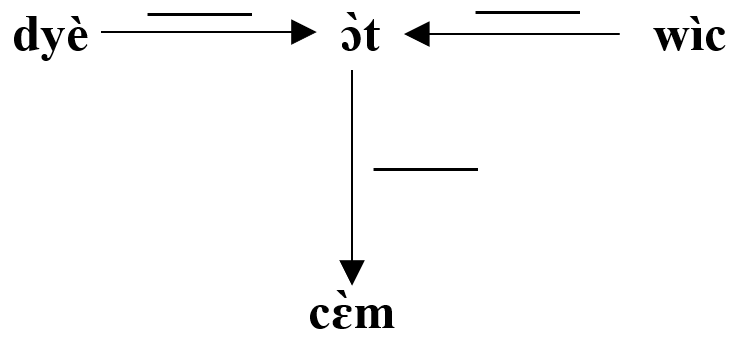
\includegraphics[width = 0.6\linewidth]{images/Lango-step1.png}
%   \label{fig:Lango-step1}
% \end{figure}


\begin{figure}
    \caption{Graph corresponding to Step 1.}
  \label{fig:Lango-step1}
  \vskip\baselineskip
  \begin{tikzpicture}
 \node (1) at (0,0) {{\cmubdata{dyè}}};
 \node (2) at (4,0) {{\cmubdata{\`{ɔ}t}}};
 \node (3) at (8,0) {\cmubdata{wìc}};
 \node (4) at (4,-2) {{\cmubdata{c\`{ɛ}m}}};
 \draw[-{Stealth[]}] (1) -- (2) node[anchor=south,inner sep=3pt,midway] {\underline{\phantom{~~~~~~~~~~~~~~~~~~}}};
 \draw[-{Stealth[]}] (3) -- (2) node[anchor=south,inner sep=3pt,midway] {\underline{\phantom{~~~~~~~~~~~~~~~~~~}}};
 \draw[-{Stealth[]}] (2) -- (4) node[inner sep=3pt,midway,right] {\underline{\phantom{~~~~~~~~~~~~~~~~~~}}};
  \end{tikzpicture}
\end{figure}


We continue to connect each word and obtain the final graphs in \figref{fig:Lango-step2}. Note that for this problem there are two independent subgraphs.

% \begin{figure}[ht]
%   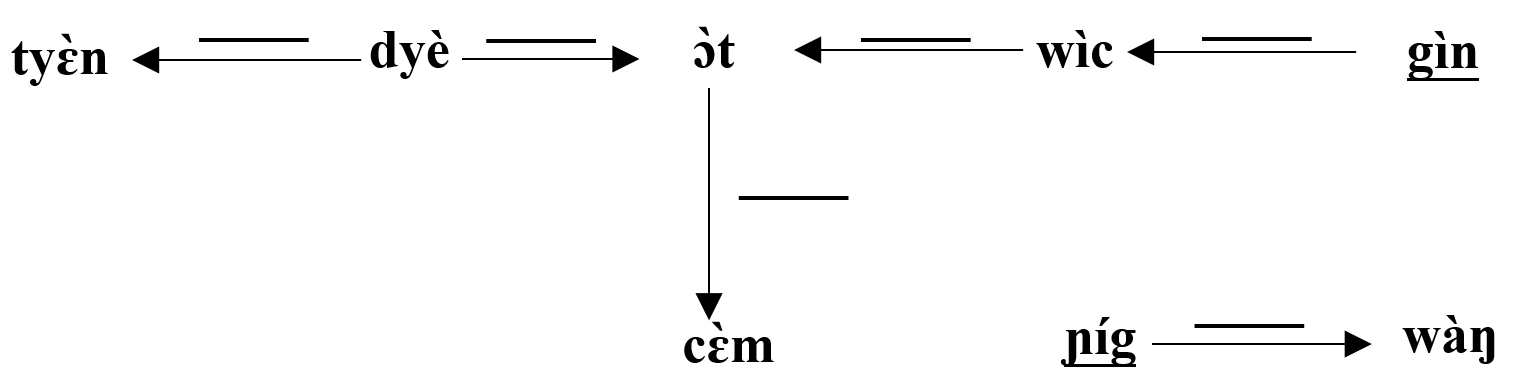
\includegraphics[width = \linewidth]{images/Lango-step2.png}
%   \caption{}
%   \label{fig:Lango-step2}
% \end{figure}

\begin{figure}
  \caption{Complete graph of the words and phrases in Lango.}
  \label{fig:Lango-step2}
  \vskip2\baselineskip
  \begin{tikzpicture}
 \node (1) at (0,0)  {{\cmubdata{dyè}}};
 \node (2) at (2.75,0)  {{\cmubdata{\`{ɔ}t}}};
 \node (3) at (5.5,0)  {{\cmubdata{wìc}}};
 \node (4) at (2.75,-2) {{\cmubdata{c\`{ɛ}m}}};
 \node (5) at (-2.75,0) {{\cmubdata{ty\`{ɛ}n}}};
 \node (6) at (8.25,0)  {{\underline{\cmubdata{gìn}}}};
 \node (7) at (5.5,-2) {{\underline{\cmubdata{ɲíg}}}};
 \node (8) at (8.25,-2) {{\cmubdata{wàŋ}}};
 \draw[-{Stealth[]}] (1) -- (2) node[anchor=south,inner sep=3pt,midway] {\underline{\phantom{~~~~~~~~~~~~~~}}};
 \draw[-{Stealth[]}] (3) -- (2) node[anchor=south,inner sep=3pt,midway] {\underline{\phantom{{~~~~~~~~~~~~~~}}}};
 \draw[-{Stealth[]}] (2) -- (4) node[anchor=south,inner sep=3pt,midway,right] {\underline{\phantom{~~~~~~~~~~~~~~}}};
 \draw[-{Stealth[]}] (1) -- (5) node[anchor=south,inner sep=3pt,midway] {\underline{\phantom{~~~~~~~~~~~~~~}}};
 \draw[-{Stealth[]}] (6) -- (3) node[anchor=south,inner sep=3pt,midway] {\underline{\phantom{~~~~~~~~~~~~~~}}};
 \draw[-{Stealth[]}] (7) -- (8) node[anchor=south,inner sep=3pt,midway] {\underline{\phantom{~~~~~~~~~~~~~~}}};
  \end{tikzpicture}
\end{figure}


 Notice that we have two separate subgraphs: the first one, which has a T-shape, and the second one which only has two nodes. Moreover, notice that the words \cmubdata{gìn} and \cmubdata{ɲíg} are underlined, meaning they also appear as single words in the corpus.

\item[Step 2.] It is time to try and form a partial graph using the English words. At first sight, we can certainly correlate the word pairs: \texttr{roof} -- \texttr{floor} (top part and bottom part of the room/house), as well as \texttr{hat} -- \texttr{roof} (the covering of the head and of the room/house). Since the word \texttr{garment} is already given, we can consider \texttr{hat} to be the \texttr{head garment\slash the garment of the top part}. Thus, we can create the partial graph shown in \figref{fig:Lango-EN-partial}.

\begin{figure}
\centering

\begin{tikzpicture}
\node (1) at (0,0) {\cmubdata{bottom}};
\node (2) at (3,0) {\cmubdata{house}};
\node (3) at (6,0) {\cmubdata{top}};
\node (4) at (9,0) {{\underline{\cmubdata{garment}}}};
\draw (1) -- (2) node[anchor=south,inner sep=3pt,midway] {\underline{\cmubdata{floor}}};
\draw (2) -- (3) node[anchor=south,inner sep=3pt,midway] {\underline{\cmubdata{roof}}};
\draw (4) -- (3) node[anchor=south,inner sep=3pt,midway] {\underline{\cmubdata{hat}}};
\end{tikzpicture}
\caption{Partial graph of the English words.}
\label{fig:Lango-EN-partial}
\end{figure}
\end{description}

We need to notice, in this case, that the connection between the nodes was not done using arrows, but lines, since the order of the constituents is not relevant.

Comparing the two graphs (Figures \ref{fig:Lango-step2} and \ref{fig:Lango-EN-partial}), notice that the partial graph  contains a chain of four words (\texttr{garment} -- \texttr{top} -- \texttr{house} -- \texttr{bottom}), and one of the end-nodes is underlined (meaning it is given in the corpus). Looking at the complete graph of Lango words (\figref{fig:Lango-step2}), we know for sure that the partial graph of English words (\figref{fig:Lango-EN-partial}) cannot be part of the small subgraph, since it only has two nodes. In the big subgraph (the T-shaped one), only one node is underlined, namely \cmubdata{gìn}. Thus, we deduce that \wordtrans{gìn}{garment}, and the four nodes (\texttr{garment} -- \texttr{top} -- \texttr{house} -- \texttr{bottom}) can either be \cmubdata{gìn} -- \cmubdata{wìc} -- \cmubdata{ɔ̀t} -- \cmubdata{dyè}, or \cmubdata{gìn} -- \cmubdata{wìc} -- \cmubdata{ɔ̀t} -- \cmubdata{cɛ̀m}. Either way, the first three words are identical, so we deduce that \wordtrans{gìn}{garment}, \wordtrans{gìn wìc}{hat}, \wordtrans{wìc}{top}, \wordtrans{wìc ɔ̀t}{roof}, \wordtrans{ɔ̀t}{house}. Following this, the proposed graph becomes the one shown in \figref{fig:Lango-step3}.
\end{mysolution}

\begin{figure}[H]
%   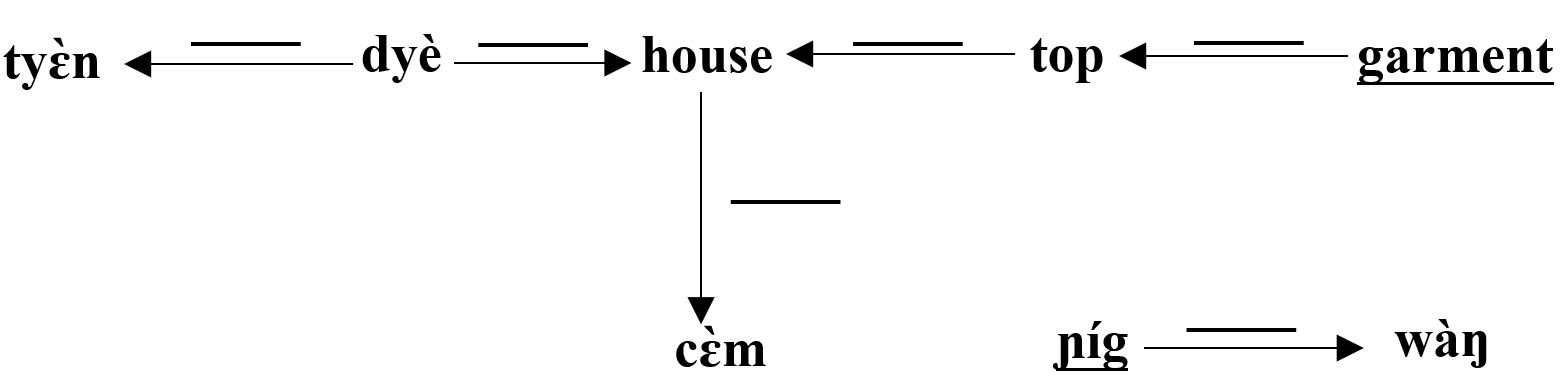
\includegraphics[width=\linewidth]{images/Lango-step-3.png}
\vskip2\baselineskip
\begin{tikzpicture}
    \node (1) at (0,0) {{\cmubdata{dyè}}};
    \node (2) at (2.75,0) {\texttr{house}};
    \node (3) at (5.5,0) {\texttr{top}};
    \node (4) at (2.75,-2) {{\cmubdata{c\`{ɛ}m}}};
    \node (5) at (-2.75,0) {{\cmubdata{ty\`{ɛ}n}}};
    \node (6) at (8.25,0) {\texttr{\underline{garment}}};
    \node (7) at (5.5,-2) {{\underline{\cmubdata{ɲíg}}}};
    \node (8) at (8.25,-2) {{\cmubdata{wàŋ}}};
    \draw[-{Stealth[]}] (1) -- (2) node[anchor=south,inner sep=3pt,midway] {\underline{\phantom{~~~~~~~~~~~~}}};
    \draw[-{Stealth[]}] (3) -- (2) node[anchor=south,inner sep=3pt,midway] {\underline{\texttr{roof}}};
    \draw[-{Stealth[]}] (2) -- (4) node[anchor=south,inner sep=3pt,midway,right] {\underline{\phantom{~~~~~~~~~~~~}}};
    \draw[-{Stealth[]}] (1) -- (5) node[anchor=south,inner sep=3pt,midway] {\underline{\phantom{~~~~~~~~~~~~}}};
    \draw[-{Stealth[]}] (6) -- (3) node[anchor=south,inner sep=3pt,midway] {\underline{\texttr{hat}}};
    \draw[-{Stealth[]}] (7) -- (8) node[anchor=south,inner sep=3pt,midway] {\underline{\phantom{~~~~~~~~~~~~}}};
\end{tikzpicture}
\caption{Partially solved graph.}
\label{fig:Lango-step3}
\end{figure}


 Moreover, we know that one of the words \cmubdata{cɛ̀m} and \cmubdata{dyè} means \texttr{bottom}.

The remaining English words are: \texttr{floor} (which we know represents \texttr{house $+$ bottom}), \texttr{grain}, \texttr{eyeball}, \texttr{restaurant}, and \texttr{sole of foot}. We can already assume that \texttr{sole of foot} is connected to \texttr{bottom} (the bottom of the foot\slash leg\slash body). Thus, if \cmubdata{cɛ̀m} is \texttr{bottom}, we would not be able to connect it to \texttr{foot}, therefore \wordtrans{dyè}{bottom} and \wordtrans{tyɛ̀n}{foot}. We can now modify the graph (see \figref{fig:Lango-step4}).

\begin{figure}[H]
% % %   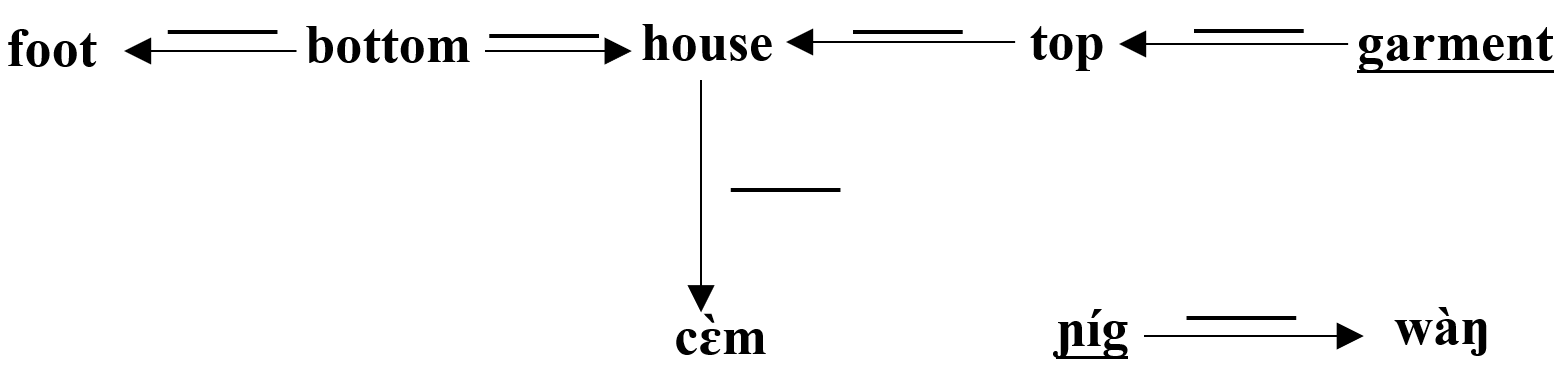
\includegraphics[width = \linewidth]{images/Lango-step4.png}
\vskip2\baselineskip
\begin{tikzpicture}
    \node (1) at (0,0)  {\texttr{bottom}};
    \node (2) at (2.75,0)  {\texttr{house}};
    \node (3) at (5.5,0)  {\texttr{top}};
    \node (4) at (2.75,-2) {{\cmubdata{c\`{ɛ}m}}};
    \node (5) at (-2.75,0) {\texttr{foot}};
    \node (6) at (8.25,0)  {\texttr{\underline{garment}}};
    \node (7) at (5.5,-2) {{\underline{\cmubdata{ɲíg}}}};
    \node (8) at (8.25,-2) {{\cmubdata{wàŋ}}};
    \draw[-{Stealth[]}] (1) -- (2) node[anchor=south,inner sep=3pt,midway] {\underline{\texttr{floor}}};
    \draw[-{Stealth[]}] (3) -- (2) node[anchor=south,inner sep=3pt,midway] {\underline{\texttr{roof}}};
    \draw[-{Stealth[]}] (2) -- (4) node[anchor=south,inner sep=3pt,midway,right] {\underline{\phantom{~~~~~~~~~~~~}}};
    \draw[-{Stealth[]}] (1) -- (5) node[anchor=south,inner sep=3pt,midway] {\underline{\texttr{sole}}};
    \draw[-{Stealth[]}] (6) -- (3) node[anchor=south,inner sep=3pt,midway] {\underline{\texttr{hat}}};
    \draw[-{Stealth[]}] (7) -- (8) node[anchor=south,inner sep=3pt,midway] {\underline{\phantom{~~~~~~~~~~~~}}};
\end{tikzpicture}
\caption{Partially solved graph, including \texttr{bottom} and \texttr{foot}.}
\label{fig:Lango-step4}
\end{figure}

 We are left with three words: \texttr{restaurant}, \texttr{eyeball}, and \texttr{grain}. Moreover, we know that one of them needs to be connected to \texttr{house} (\texttr{house} $+$ \cmubdata{cɛ̀m}), while the other two must be derived from one another (\cmubdata{ɲíg} and \cmubdata{ɲíg wàŋ}). Among the English words, the one which is most closely related semantically with \texttr{house} is \texttr{restaurant} (\texttr{restaurant} $=$ \texttr{house} $+$ \texttr{food}), while \texttr{eyeball} can be derived from \texttr{grain} as in \texttr{eyeball} $=$ \texttr{grain} $+$ \texttr{eye} (the grain of the eye).

Thus, we can make all the correspondences:
\begin{mysolution}
\begin{assgts}
    \item 
    \begin{tabular}[t]{lcll}
        \cmubdata{dyè ɔ̀t} & = &\texttr{floor} & (bottom + house) \\
        \cmubdata{dyè tyɛ̀n} & = &\texttr{sole of foot} & (bottom + foot) \\
        \cmubdata{gìn} & = &\texttr{garment} & \\
        \cmubdata{gìn wìc} & = &\texttr{hat} & (garment + top) \\
        \cmubdata{ɲíg} & = &\texttr{grain} &  \\
        \cmubdata{ɲíg wàŋ} & = &\texttr{eyeball} & (grain + eye) \\
        \cmubdata{ɔ̀t cɛ̀m} & = &\texttr{restaurant} & (house + food) \\
        \cmubdata{wìc ɔ̀t} & = &\texttr{roof} & (top + house) \\
    \end{tabular}
\item \begin{tabular}[t]{lcl} \cmubdata{cɛ̀m} & = & \texttr{food} \\
                               \cmubdata{dyè} & = & \texttr{bottom}\\
      \end{tabular}
\end{assgts}

 For task (c), we need to use the words we already have. Thus, we deduce that \texttr{window} $=$ eye of the house $=$ \texttr{eye} $+$ \texttr{house} (we deduce the word order from the phrase \texttr{eyeball} $=$ grain of the eye $=$ \texttr{grain} $+$ \texttr{eye}, and not *\texttr{eye} $+$ \texttr{grain}). Thus, \texttr{window} = \cmubdata{wàŋ ɔ̀t}.

This is, however, an easy problem for which a graph is not necessarily needed, since one can observe that the only word which occurs in three different phrases is \cmubdata{ɔ̀t}, and the only three English translations which have something in common are \texttr{floor}, \texttr{roof}, and \texttr{restaurant} (they are connected to a house\slash building). Nevertheless, the problem above offers an easy-to-understand example for the way in which graphs can be used to solve this type of problem.

We can now try to apply this method to solving a more complex problem.
\end{mysolution}

\pagebreak
\begin{problem}{\langnameGuarani}{\nameASouza}{\LOYear{\RoLOAbbr}{2021}}
\IntroWordComb{\langnameGuarani}\ \IntroAndEnglishRandom:

\begin{center}
    \begin{longtable}{rl@{\hskip0.5in}cl}
       \chaosline{jaxy}{water}
       \chaosline{jaxy-tata}{brave}
       \chaosline{jaxy endy}{thumb}
       \chaosline{kuã guaxu}{liver, heart}
       \chaosline{kuã regua}{fire}
       \chaosline{py'a}{smoke}
       \chaosline{py'a guaxu}{pregnant}
       \chaosline{tata}{ring (jewellery)}
       \chaosline{tata endy}{moonlight}
       \chaosline{tata rataxĩ}{firelight}
       \chaosline{ye guaxu}{moon}
       \chaosline{yvy rataxĩ}{good soil}
       \chaosline{yvy porã}{dust}
       \chaosline{yy}{star}
    \end{longtable}
\end{center}

\begin{assgts}
\item \detcorr
\item \transinen
\begin{multicols}{3}
\begin{enumerate}[start = 15]
    \item \cmubdata{guaxu}
    \item \cmubdata{porã} 
    \item \cmubdata{rataxĩ}
    \item \cmubdata{regua}
    \item \cmubdata{ye}
\end{enumerate}
\end{multicols}
\item \transinen[\langnameGuarani]
\begin{multicols}{3}
\begin{enumerate}[start = 20]
    \item \texttr{calm, relaxed}
    \item \texttr{fog}
    \blankitem
\end{enumerate}
\end{multicols}
\end{assgts}
\end{problem}

\begin{mysolution}


 First notice that in English we have words referring to organs (\texttr{liver, heart}) and emotions (\texttr{brave} and, in task (c), \texttr{calm}). So we can expect that these two are connected. Nevertheless, the first step is constructing the graphs for the Guaraní words (see \figref{fig:Guarani-step1}).

% \begin{figure}[ht]
%   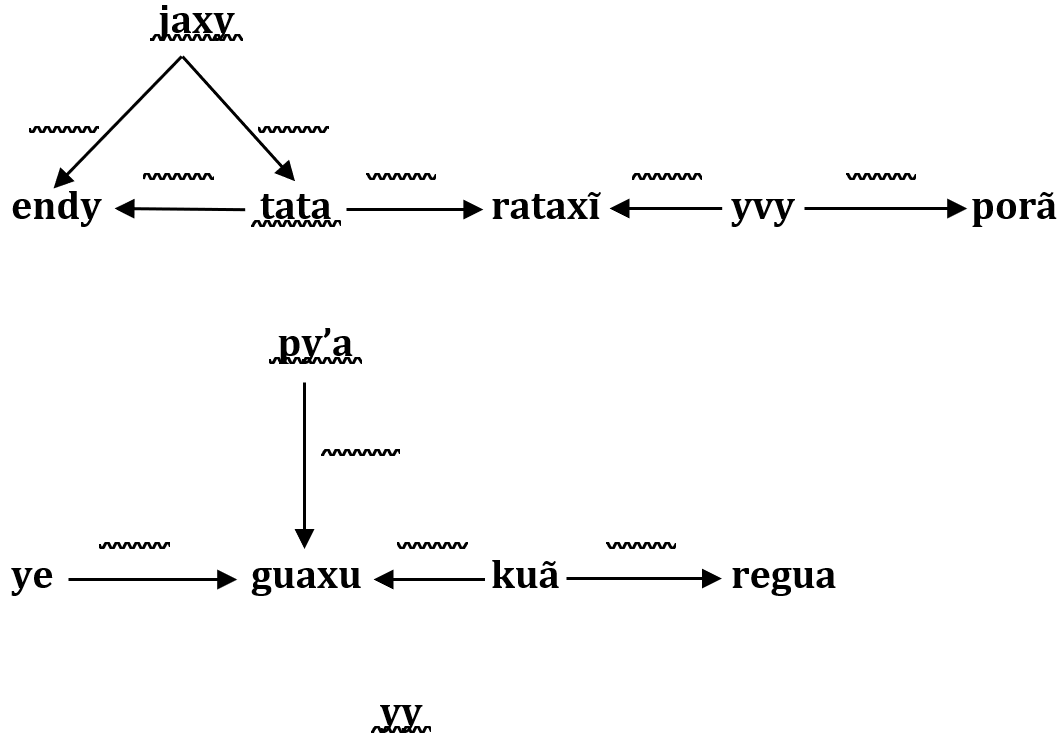
\includegraphics[width = 0.8\linewidth]{images/Guarani-1.png}
% \end{figure}

\begin{figure}[H]
\caption{Complete graph of the words and phrases in Guaraní.}
\label{fig:Guarani-step1}
%   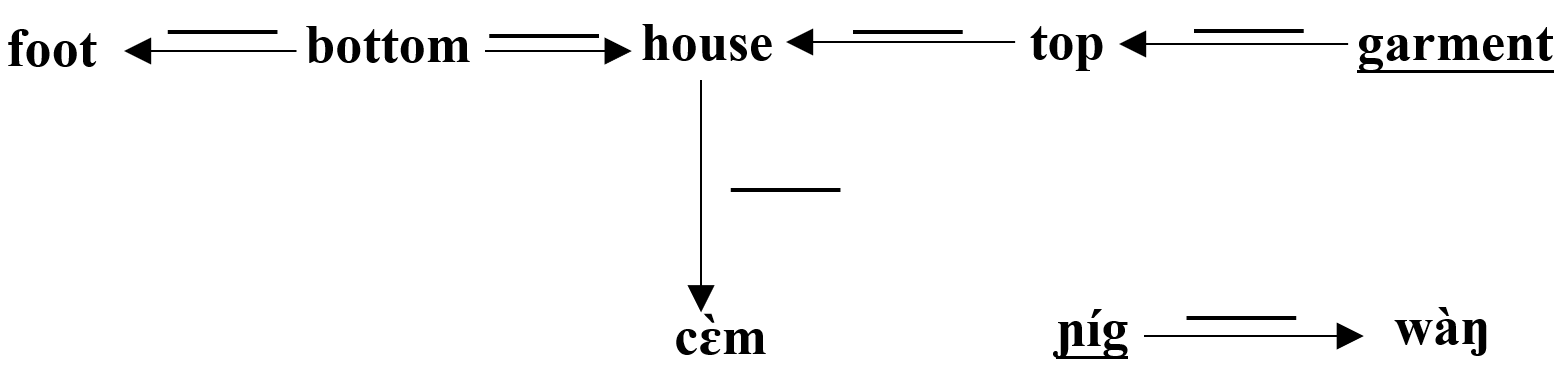
\includegraphics[width = \linewidth]{images/Lango-step4.png}
\begin{tikzpicture}
    \node (1) at (0,0) {\cmubdata{endy}};
    \node (2) at (2,0) {\uwave{\cmubdata{tata}}};
    \node (3) at (4,0) {\cmubdata{rataxĩ}};
    \node (4) at (6,0) {\cmubdata{yvy}};
    \node (5) at (8,0) {\cmubdata{porã}};
    \node (6) at (1,2) {\uwave{\cmubdata{jaxy}}};
    \draw[-{Stealth[]}] (2) -- (1) node[anchor=south,inner sep=3pt,midway] {\uwave{\phantom{~~~~~~}}};
    \draw[-{Stealth[]}] (2) -- (3) node[anchor=south,inner sep=3pt,midway] {\uwave{\phantom{~~~~~~}}};
    \draw[-{Stealth[]}] (4) -- (3) node[anchor=south,inner sep=3pt,midway] {\uwave{\phantom{~~~~~~}}};
    \draw[-{Stealth[]}] (5) -- (4) node[anchor=south,inner sep=3pt,midway] {\uwave{\phantom{~~~~~~}}};
    \draw[-{Stealth[]}] (6) -- (1) node[anchor=south,inner sep=3pt,midway,left] {\uwave{\phantom{~~~~~~}}};
    \draw[-{Stealth[]}] (6) -- (2) node[anchor=south,inner sep=3pt,midway,right] {\uwave{\phantom{~~~~~~}}};
\end{tikzpicture}
  
\begin{tikzpicture}
    \node (1) at (0,0) {\cmubdata{ye}};
    \node (2) at (2,0) {\cmubdata{guaxu}};
    \node (3) at (4,0) {\cmubdata{kuã}};
    \node (4) at (6,0) {\cmubdata{regua}};
    \node (5) at (3,-1.5) {\uwave{\cmubdata{yy}}};
    \node (6) at (2,2) {\uwave{\cmubdata{py'a}}};
    \draw[-{Stealth[]}] (1) -- (2) node[anchor=south,inner sep=3pt,midway] {\uwave{\phantom{~~~~~~}}};
    \draw[-{Stealth[]}] (3) -- (2) node[anchor=south,inner sep=3pt,midway] {\uwave{\phantom{~~~~~~}}};
    \draw[-{Stealth[]}] (3) -- (4) node[anchor=south,inner sep=3pt,midway] {\uwave{\phantom{~~~~~~}}};
    \draw[-{Stealth[]}] (6) -- (2) node[anchor=south,inner sep=3pt,midway,right] {\uwave{\phantom{~~~~~~}}};
\end{tikzpicture}
\end{figure}


\note{In Appendix~\ref{appendix:3} I present a hand-drawn graph in order to show what such a graph might look like in reality, when solving a problem.}


We notice that, in Guaraní, we have three independent subgraphs. For the partial graph of English words, we have the words: \texttr{moon}, \texttr{fire}, \texttr{moonlight}, and \texttr{firelight}. These can be arranged in a graph as shown in \figref{fig:Guarani-step2}.

% \begin{figure}[ht]
%   \caption{}

% \end{figure}

\begin{figure}[H]
% 
\includegraphics[width = 0.4\linewidth]{images/Guarani-2.png}
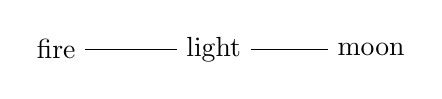
\begin{tikzpicture}
\node (1) at (2,0) {\uwave{\texttr{fire}}};
\node (2) at (4,0) {\texttr{light}};
\node (3) at (6,0) {\uwave{\texttr{moon}}};
\draw (1) -- (2) node[anchor=south,inner sep=3pt,midway] {\uwave{{~~~~~~}}};
\draw (2) -- (3) node[anchor=south,inner sep=3pt,midway] {\uwave{{~~~~~~}}};
\end{tikzpicture}
\caption{Partial graph of the English words \texttr{moon}, \texttr{fire}, \texttr{moonlight}, and \texttr{firelight}.}
\label{fig:Guarani-step2}
\end{figure}



 This is an ideal partial graph since we have two base words (nodes), \texttr{fire}, and \texttr{moon}, which are found in the corpus and are both connected to the same word (\texttr{light}). According to the Guaraní graph in \figref{fig:Guarani-step1}, the only two nodes close to one another that are found in the corpus (are underlined) are \cmubdata{jaxy} and \cmubdata{tata}, and both of them are connected to the word \cmubdata{endy}. Thus, we deduce that \wordtrans{endy}{light}, and \{\cmubdata{jaxy}, \cmubdata{tata}\} = \{\texttr{fire}, \texttr{moon}\}\footnote{By this notation, we mean that \cmubdata{jaxy} and \cmubdata{tata} correspond to \texttr{fire} and \texttr{moon}, but we do not know which is which.}. In order to determine which is which, we notice that \cmubdata{jaxy} is not connected to anything else, while \cmubdata{tata} is further connected to \cmubdata{rataxĩ}. In English, we have the word \texttr{smoke} which is clearly connected to \texttr{fire}, so \wordtrans{tata}{fire} and \wordtrans{jaxy}{moon}. Moreover, from the graph, we notice that \cmubdata{jaxy} and \cmubdata{tata} combine with one another, thus, in English, we need to find a word formed by combining the words \texttr{moon} and \texttr{fire}. The only one which is semantically close to that is \texttr{star} ( = \texttr{fire moon}). Adding this information, our graph will look like that in \figref{fig:Guarani-step3}.

\begin{figure}
  \caption{Partially solved graph.}
\label{fig:Guarani-step3}
% %   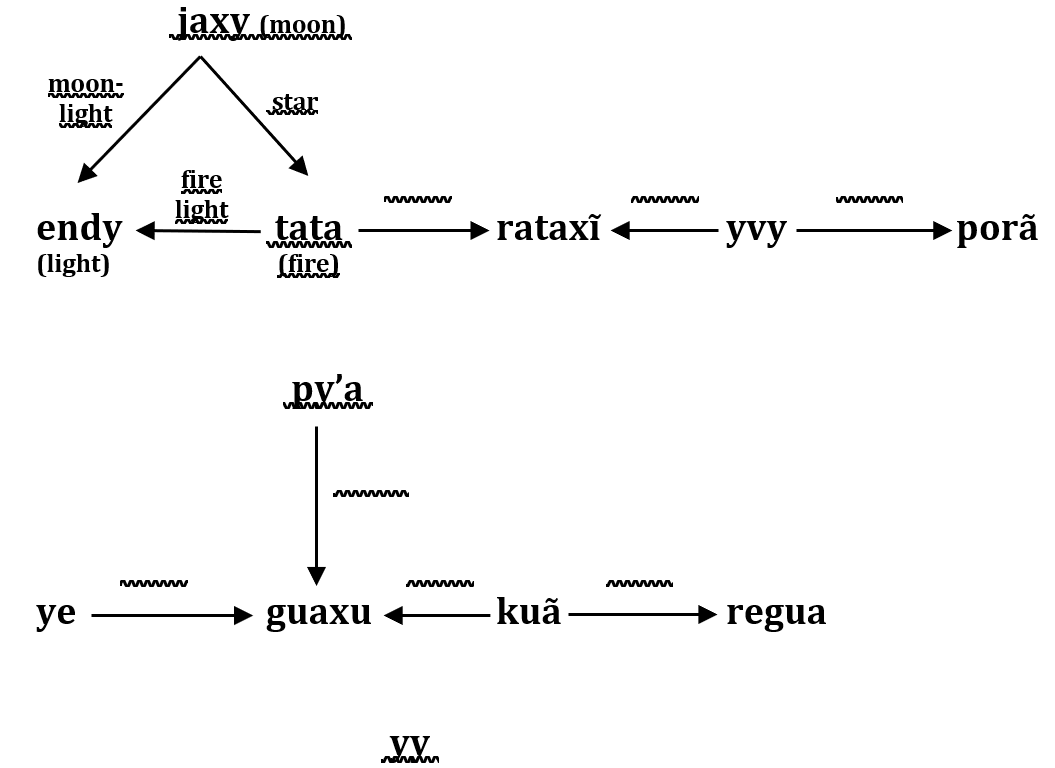
\includegraphics[width = \linewidth]{images/Guarani-3.png}
  \begin{tikzpicture}[every node/.style={align=center}]
    \node (1) at (0,0) {\cmubdata{endy}\\(\texttr{light})};
    \node (2) at (3,0) {\uwave{\cmubdata{tata}}\\(\texttr{fire})};
    \node (3) at (6,0) {\cmubdata{rataxĩ}};
    \node (4) at (8,0) {\cmubdata{yvy}};
    \node (5) at (10,0) {\cmubdata{porã}};
    \node (6) at (1.5,2) {\uwave{\cmubdata{jaxy}}\\ (\texttr{moon})};
    \draw[-{Stealth[]}] (2) -- (1) node[anchor=south,inner sep=3pt,midway] {\uwave{\texttr{firelight}}};
    \draw[-{Stealth[]}] (2) -- (3) node[anchor=south,inner sep=3pt,midway] {\uwave{\texttr{smoke}}};
    \draw[-{Stealth[]}] (4) -- (3) node[anchor=south,inner sep=3pt,midway] {\uwave{\phantom{~~~~~~}}};
    \draw[-{Stealth[]}] (5) -- (4) node[anchor=south,inner sep=3pt,midway] {\uwave{\phantom{~~~~~~}}};
    \draw[-{Stealth[]}] (6) -- (1) node[anchor=south,inner sep=3pt,midway,left] {\uwave{\texttr{moonlight}}};
    \draw[-{Stealth[]}] (6) -- (2) node[anchor=south,inner sep=3pt,midway,right] {\uwave{\texttr{star}}};
\end{tikzpicture}\bigskip\\  
\begin{tikzpicture}[every node/.style={align=center}]
  \node (1) at (0,0) {\cmubdata{ye}};
  \node (2) at (3,0) {\cmubdata{guaxu}};
  \node (3) at (6,0) {\cmubdata{kuã}};
  \node (4) at (9,0) {\cmubdata{regua}};
  \node (5) at (4.5,-1.5) {\uwave{\cmubdata{yy}}};
  \node (6) at (3,2) {\uwave{\cmubdata{py'a}}};
  \draw[-{Stealth[]}] (1) -- (2) node[anchor=south,inner sep=3pt,midway] {\uwave{\phantom{~~~~~~}}};
  \draw[-{Stealth[]}] (3) -- (2) node[anchor=south,inner sep=3pt,midway] {\uwave{\phantom{~~~~~~}}};
  \draw[-{Stealth[]}] (3) -- (4) node[anchor=south,inner sep=3pt,midway] {\uwave{\phantom{~~~~~~}}};
  \draw[-{Stealth[]}] (6) -- (2) node[anchor=south,inner sep=3pt,midway,right] {\uwave{\phantom{~~~~~~}}};
\end{tikzpicture}
\end{figure}


 As mentioned above, \texttr{fire} is only combined with one more word and, in English, the only word that belongs to the same semantic field is \texttr{smoke}. Thus, \wordtrans{tata rataxĩ}{smoke}. Nevertheless, we cannot immediately deduce the meaning of \cmubdata{rataxĩ} (\texttr{smoke} = \texttr{fire} $+$ $X$). However, looking at the English words, we notice the word \texttr{dust} and, since this roughly relates to the same semantic area as \texttr{smoke}, they most likely have something in common (the word $X$). Thus, we get:

\begin{exe}
 \sn[]{\texttr{smoke} = \texttr{fire} $+$ $X$ \quad\quad\quad\quad and \quad\quad\quad\quad \texttr{dust} = ? $+$ $X$}
\end{exe}

Comparing again the remaining words, we notice we have the phrase \texttr{good soil} (and, indeed, \texttr{smoke} is to \texttr{fire} as \texttr{dust} is to \texttr{soil}). Therefore, $X$ represents \texttr{particles/powder} (smoke is a ``powder'' from the fire, while dust is a powder of soil). Thus, we can complete the top subgraph as shown in \figref{fig:Guarani-step4}.

\begin{figure}
% % %   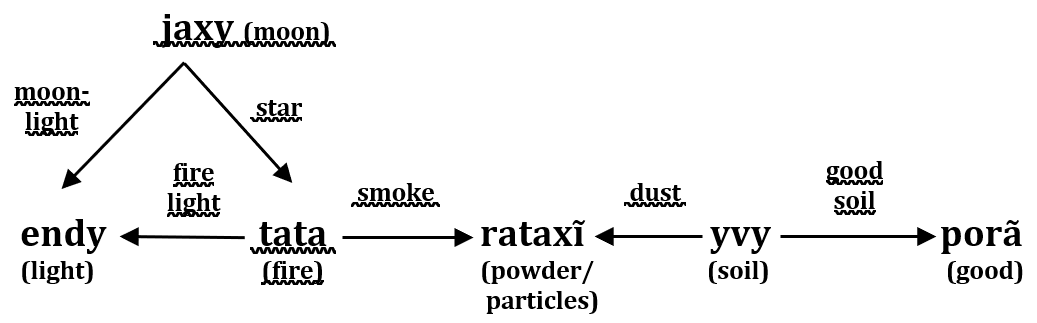
\includegraphics[width = 0.9\linewidth]{images/Guarani-4.png}
\caption{Completely solved top subgraph.}
\label{fig:Guarani-step4}
\begin{tikzpicture}[every node/.style={align=center}]
    \node (1) at (0,0) {\cmubdata{endy}\\ (\texttr{light})};
    \node (2) at (3,0) {\uwave{\cmubdata{tata}} \\ (\texttr{fire})};
    \node (3) at (6,0) {\cmubdata{rataxĩ}\\ (\texttr{powder}/\\ \texttr{particles})};
    \node (4) at (8,0) {\cmubdata{yvy}\\ (\texttr{soil})};
    \node (5) at (10,0) {\cmubdata{porã}\\ (\texttr{good})};
    \node (6) at (1.5,2) {\uwave{\cmubdata{jaxy}}\\ (\texttr{moon})};
    \draw[-{Stealth[]}] (2) -- (1) node[anchor=south,inner sep=3pt,midway] {\uwave{\texttr{firelight}}};
    \draw[-{Stealth[]}] (2) -- (3) node[anchor=south,inner sep=3pt,midway] {\uwave{\texttr{smoke}}};
    \draw[-{Stealth[]}] (4) -- (3) node[anchor=south,inner sep=3pt,midway] {\uwave{\texttr{dust}}};
    \draw[-{Stealth[]}] (5) -- (4) node[anchor=south,inner sep=3pt,midway] {\texttr{good\\ \uwave{soil}}};
    \draw[-{Stealth[]}] (6) -- (1) node[anchor=south,inner sep=3pt,midway,left] {\uwave{\texttr{moonlight}}};
    \draw[-{Stealth[]}] (6) -- (2) node[anchor=south,inner sep=3pt,midway,right] {\uwave{\texttr{star}}};
\end{tikzpicture}
\end{figure}

Since this subgraph is independent (not connected to the others in any way), we have reached a dead end and we need to build a new partial graph based on the English words. However, we have already made eight correspondences. The remaining words are:

\begin{center}
\begin{tabular}{rl@{\hskip0.5in}cl}
      4. & \cmubdata{kuã guaxu} & A. & \texttr{water} \\
      5. & \cmubdata{kuã regua} & B. & \texttr{brave} \\
      6. & \cmubdata{py'a} & C. & \texttr{thumb} \\
      7. & \cmubdata{py'a guaxu} & D. & \texttr{liver, heart} \\
      11. & \cmubdata{ye guaxu} & G. & \texttr{pregnant} \\
      14. & \cmubdata{yy} & H. & \texttr{ring} \\
\end{tabular}
\end{center}


Among these, we can notice \texttr{ring} and \texttr{thumb} (both being related to the word \texttr{finger}, as in \texttr{thumb} = \texttr{finger} + \texttr{big} and \texttr{ring} = \texttr{finger} + \texttr{jewellery/ornament}). Only based on these two words, we can build the graph shown in \figref{fig:Guarani-step5}.

\begin{figure}[H]
%   
\includegraphics[width =.5\linewidth]{images/Guarani-5.png}
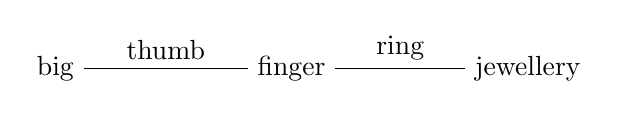
\begin{tikzpicture}[every node/.style={align=center}]
    \node (1) at (2,0) {{\texttr{big}}};
    \node (2) at (5,0) {\texttr{finger}};
    \node (3) at (8,0) {{\texttr{jewellery}}};
    \draw (1) -- (2) node[anchor=south,inner sep=3pt,midway] {\uwave{\texttr{thumb}}};
    \draw (2) -- (3) node[anchor=south,inner sep=3pt,midway] {\uwave{\texttr{ring}}};
\end{tikzpicture}
\caption{Partial graph.}
\label{fig:Guarani-step5}
\end{figure}

 Thus, \texttr{finger} can correspond to either \cmubdata{kuã}, or \cmubdata{guaxu}. If it corresponded to \cmubdata{guaxu}, it needs to combine with another word among those given (i.e., \texttr{finger} $+$ \texttr{water}, \texttr{finger} $+$ \texttr{brave}, \texttr{finger} $+$ \texttr{liver, heart}, \texttr{finger} $+$ \texttr{pregnant}), all of these combinations being highly unlikely (difficult to justify). Therefore, \wordtrans{kuã}{finger}. Moreover, we notice that no other word seems to belong in the semantic field of the word \texttr{jewellery, ornament}, so, most likely this is the meaning of \cmubdata{regua}. The graph now looks like that shown in \figref{fig:Guarani-step6}.
 
\begin{figure}
%   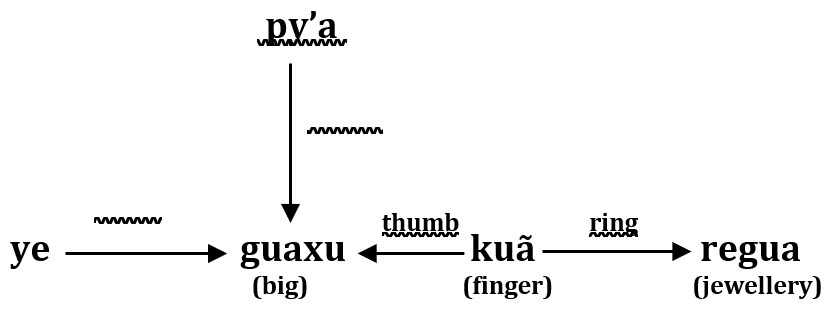
\includegraphics[width = 0.7\linewidth]{images/Guarani-6.png}
\caption{Completely solved subgraph.}
\label{fig:Guarani-step6}
\begin{tikzpicture}[every node/.style={align=center}]
    \node (1) at (0,0) {\cmubdata{ye}};
    \node (2) at (3,0) {\cmubdata{guaxu}\\ (\texttr{big})};
    \node (3) at (6,0) {\cmubdata{kuã}\\(\texttr{finger})};
    \node (4) at (10,0) {\cmubdata{regua}\\(\texttr{jewellery})};
    \node (5) at (3,2) {\uwave{\cmubdata{py'a}}};
    \draw[-{Stealth[]}] (1) -- (2) node[anchor=south,inner sep=3pt,midway] {\uwave{\phantom{~~~~~~}}};
    \draw[-{Stealth[]}] (3) -- (2) node[anchor=south,inner sep=3pt,midway] {\uwave{\texttr{thumb}}};
    \draw[-{Stealth[]}] (3) -- (4) node[anchor=south,inner sep=3pt,midway] {\uwave{\texttr{ring}}};
    \draw[-{Stealth[]}] (5) -- (2) node[anchor=south,inner sep=3pt,midway,right] {\uwave{\phantom{~~~~~~}}};
\end{tikzpicture}
\end{figure}

We need to have in the corpus two more words which are formed from the combination of \texttr{big} with other words (and one of the words it combines with -- \cmubdata{py'a} -- must also appear in the corpus). The first word we notice is \texttr{pregnant} (we can consider that it is formed as \texttr{belly} $+$ \texttr{big} or something similar). Moreover, we notice that we have \texttr{liver, heart} and \texttr{brave} among the remaining words. As mentioned above, words for emotions are often formed from words designating organs, so \texttr{brave} = \texttr{big} $+$ \texttr{heart, liver} is quite plausible. In this way, we also completed this subgraph and the only remaining word, \cmubdata{yy}, must mean \texttr{water}.

So we have the correspondences:


\begin{center}
    \begin{tabular}{rlcll}
         1. & \cmubdata{jaxy} & = & \texttr{moon} &  \\
         2. & \cmubdata{jaxy-tata} & = & \texttr{star} & (moon + fire) \\
         3. & \cmubdata{jaxy endy} & = & \texttr{moonlight} &  \\
         4. & \cmubdata{kuã guaxu} & = & \texttr{thumb} & (finger + big) \\
         5. & \cmubdata{kuã regua} & = & \texttr{ring} & (finger + jewellery) \\
         6. & \cmubdata{py'a} & = & \texttr{liver, heart} &  \\
         7. & \cmubdata{py'a guaxu} & = & \texttr{brave} & (liver, heart + big) \\
         8. & \cmubdata{tata} & = & \texttr{fire} &  \\
         9. & \cmubdata{tata endy} & = & \texttr{firelight} &  \\
         10. & \cmubdata{tata rataxĩ} & = & \texttr{smoke} & (fire + powder) \\
         11. & \cmubdata{ye guaxu} & = & \texttr{pregnant} & (belly + big) \\
         12. & \cmubdata{yvy rataxĩ} & = & \texttr{dust} & (soil + powder) \\
         13. & \cmubdata{yvy porã} & = & \texttr{good soil} & (soil + good)  \\
         14. & \cmubdata{yy} & = & \texttr{water} &  \\
    \end{tabular}
\end{center}


In task (b), we are only asked to translate simple words (which correspond to the nodes of the graph), so this task is straightforward now: \wordtrans{guaxu}{big}, \wordtrans{porã}{good}, \wordtrans{rataxĩ}{powder}, \wordtrans{regua}{ornament/jewellery}, \wordtrans{ye}{belly}.

\remember{For this type of problem, there might be multiple acceptable answers, which is taken into account when grading. Thus, for the word \cmubdata{regua} (which must be deduced from the combination \texttr{ring} = \texttr{finger} $+$ \cmubdata{regua}), there can be multiple interpretations: \texttr{ornament}, \texttr{jewellery} etc., but it can also be considered to mean \texttr{circle}, \texttr{surrounding}, etc. (which is the actual meaning of the Guaraní word). Thus, all of these words would be equally acceptable.}

 In task (c), we are asked to translate the words \texttr{fog} and \texttr{calm}. The word \texttr{fog} is easy to translate since it resembles \texttr{dust} and \texttr{smoke} (thus, \texttr{fog} = \texttr{water} $+$ \texttr{powder}), so its translation is \cmubdata{yy rataxĩ}. The word \texttr{calm} can be compared with the word \texttr{brave} (both referring to human qualities). Since \texttr{brave} was formed from \texttr{liver, heart}, it is likely that \texttr{calm} is too. Moreover, we notice that we also have another adjective: \texttr{good}. Therefore, we can form the combination \texttr{calm} = \texttr{good} + \texttr{liver, heart}. Thus, its translation is \cmubdata{py'a porã}.



Put all together, the answers are:

\begin{assgts}
    \item
    \begin{enumerate}
    \begin{multicols}{7}
        \item K.
        \item N.
        \item I.
        \item C.
        \item H.
        \item D.
        \item B.
        \item E.
        \item J.
        \item F.
        \item G.
        \item M.
        \item L.
        \item A.
        \end{multicols}
    \end{enumerate}
    \item
    \begin{enumerate}[start = 15]
    \begin{multicols}{2}
        \item \texttr{big}
        \item \texttr{good}
        \item \texttr{powder, particles}
        \item \texttr{circle}
        \item \texttr{belly, stomach}
        \item[] \hphantom{x}
        \end{multicols}
    \end{enumerate}

    \item
    \begin{enumerate}[start = 20]
    \begin{multicols}{2}
        \item \cmubdata{py'a porã}
        \item \cmubdata{yy rataxĩ}
        \end{multicols}
    \end{enumerate}
\end{assgts}
\end{mysolution}


\hypertarget{practice-problems}{%
\section{Practice problems}}

\begin{problem}{\langnameBasque}{\nameNZaika}{\LOYear{\MSKAbbr}{2012}}
\IntroWords{\langnameBasque}\ \IntroAndEnglishRandom:

\begin{exe}
\sn[]{\cmubdata{igogailu}, \cmubdata{artzain}, \cmubdata{lantegi}, \cmubdata{lantalde}, \cmubdata{bizitegi}, \cmubdata{taldekide}, \cmubdata{erizain}, \cmubdata{garbigailu}, \cmubdata{ikastalde}, 
      \cmubdata{bizikide}, \cmubdata{garbitegi}, \cmubdata{ikaskide}, \cmubdata{lankide}, \cmubdata{eritegi}, \cmubdata{artalde}
\glt \texttr{classmate}, \texttr{flatmate}, \texttr{flock of sheep}, \texttr{crew}, \texttr{elevator}, \texttr{clinic}, \texttr{factory}, \texttr{nurse}, \texttr{home}, \texttr{shepherd},         
     \texttr{wash-house}, \texttr{colleague}, \texttr{washing machine}, \texttr{team member}, \texttr{class (of students)}}
\end{exe}

\begin{assgts}
\item \detcorr
\item How is the word \cmubdata{artalde} different from the other Basque words?
\item Translate the word \texttr{sheep-pen} into Basque, knowing that it has the same feature as the word \cmubdata{artalde}.
\end{assgts}
\end{problem}



\begin{problem}{\langnameTurkish}{\nameMChoudhury}{\LOYear{\PLOAbbr}{2014}}
\IntroWords{\langnameTurkish}\ \IntroAndEnglishRandom:

\begin{exe}\sloppy
\sn[]{\cmubdata{gözlemci}, \cmubdata{döndürmek}, \cmubdata{gündöndü}, \cmubdata{gözlükcü}, \cmubdata{şarkıcı}, \cmubdata{çocukluk}, \cmubdata{gözlemek}, \cmubdata{pazar}, \cmubdata{pazartesi}, \cmubdata{cumartesi}, \cmubdata{güneşli}
\glt \texttr{Saturday}, \texttr{Sunday}, \texttr{Monday}, \texttr{observer}, \texttr{singer}, \texttr{to observe}, \texttr{to rotate}, \texttr{sunny}, \texttr{sunflower}, \texttr{optician}, \texttr{childhood}}
\end{exe}

\begin{assgts}
\item \detcorr
\item \transinen[\langnameTurkish]
\begin{enumerate}
    \item \texttr{observation}
    \item \texttr{child}
    \item \texttr{the state of being a singer}
    \item \texttr{spectacles}
    \item \texttr{Friday}
    \blankitem
\end{enumerate}
\end{assgts}
\end{problem}

\begin{problem}{\langnameChinese}{\nameRDinca}{\LOYear{\RoLOAbbr}{2015}}
\IntroWordComb{\langnameChinese}\ \IntroAndEnglishRandom:

\begin{exe}
\sn[]{\cmubdata{hóng}, \cmubdata{míngbái}, \cmubdata{báishì}, \cmubdata{huáng}, \cmubdata{hēishì}, \cmubdata{shìqing huángle}, \cmubdata{yăn}, \cmubdata{yănhóng}, \cmubdata{hóngshì}, \cmubdata{hóngyán}, \cmubdata{hēihuà}, \cmubdata{báiyăn}, \cmubdata{báihuà}, \cmubdata{hēibái fēnmíng}, \cmubdata{yán}, \cmubdata{hēibái}, \cmubdata{huángle}
\glt \texttr{encoding}, \texttr{black-and-white}, \texttr{face}, \texttr{yellow}, \texttr{funeral}, \texttr{bankruptcy}, \texttr{to clarify}, \texttr{to dislike}, \texttr{young woman}, \texttr{failure}, \texttr{decoding}, \texttr{wedding}, \texttr{eye}, \texttr{black market}, \texttr{it's written in black and white}, \texttr{jealousy}, \texttr{red}}
\end{exe}

\begin{assgts}
\item \detcorr
\item The word \cmubdata{báishì} can have two meanings in Chinese, although only one is reflected in the correspondences above. What is the other meaning? 
\end{assgts}
\end{problem}



\begin{problem}{\langnameHausa}{\namePHelmer}{\LOYear{\RoLOAbbr}{2019}}
\IntroPhrases{\langnameHausa}\ \IntroAndEnglishRandom:

\begin{table}[H]
    \begin{tabular}{rl@{\hskip0.5in}cl}
       \chaosline{bàakín rúwáa}{talkative boy}
       \chaosline{bàbbán bàakín tsúntsúu}{white camel}
       \chaosline{bàbbán yátsàa}{big beak}
       \chaosline{bàbbán ràkúmín rúwáa}{thumb}
       \chaosline{bàbbán yár sháanúu}{fruit}
       \chaosline{bákín cíkìi}{fork}
       \chaosline{bákín ràagóo}{pregnant woman}
       \chaosline{cóokàlíi mài yátsàa}{sorrow}
       \chaosline{dán ràagóo}{estuary}
       \chaosline{dán mài bàbbán bàakíi}{lamb}
       \chaosline{fárin ràkúmíi}{black sheep}
       \chaosline{rúwán bíshíyàa}{(tree) sap}
       \chaosline{yár mài bàbbán cíkìi}{tsunami}
       \chaosline{yár bíshíyàa}{big heifer}
    \end{tabular}
\end{table}

\begin{assgts}
\item \detcorr
\item \transinen
\begin{multicols}{2}
\begin{enumerate}[start = 15]
    \item \cmubdata{dán sháanúu}
    \item \cmubdata{fárín cíkìi} 
    \item \cmubdata{yár mài bákin bàakíi} 
\end{enumerate}
\end{multicols}
\item \transinen[\langnameHausa]
\begin{multicols}{2}
\begin{enumerate}[start = 18]
    \item \texttr{girl who has a spoon}
    \item \texttr{crow}
    \item \texttr{river}
    \item \texttr{(tree) branch}

\end{enumerate}
\end{multicols}

\end{assgts}

\begin{tblsWarning}
An \texttr{estuary} is a wide part of the river, similar to a funnel. A \texttr{heifer} is a young female cow. 
\end{tblsWarning}
\end{problem}



\begin{problem}{\langnameTetum}{\nameAPegusevs}{\LOYear{\RoLOAbbr}{2020}}
\IntroWordComb{\langnameTetum}\ \IntroAndEnglishRandom:

\begin{table}[H]
    \begin{tabular}{rl@{\hskip0.5in}cl}
       \chaosline{ai boot}{eyelid}
       \chaosline{ai fuan boot}{scapula}
       \chaosline{ai fuan musan}{leaf}
       \chaosline{ai tahan}{big fruit}
       \chaosline{ibun kulit boot}{big tree}
       \chaosline{kbas}{auricle}
       \chaosline{kbas tahan}{skin}
       \chaosline{kulit}{seed}
       \chaosline{matan kulit}{shoulder}
       \chaosline{matan musan}{eyeball}
       \chaosline{tilun tahan}{big lip}
    \end{tabular}
\end{table}

\begin{assgts}
\item \detcorr
\pagebreak
\item \transinen
\begin{multicols}{3}
\begin{enumerate}[start = 12]
    \item \cmubdata{matan fuan}
    \item \cmubdata{ai fuan kulit} 
    \item \cmubdata{tilun boot} 
\end{enumerate}
\end{multicols}
\item[] One of the phrases has the same translation as one of the phrases 1--11.
\item \transinen[\langnameTetum]
\begin{multicols}{2}
\begin{enumerate}[start = 15]
    \item \texttr{mouth}
    \item \texttr{big eye}
    \item \texttr{(tree) bark}
    \item \texttr{grain}
\end{enumerate}
\end{multicols}
\item Two of the words above can be combined to construct a phrase meaning \texttr{impolite person}. Which ones are these? 
\end{assgts}

\begin{tblsWarning}
The \texttr{scapula} (or shoulder blade) is the large flat bone that is part of the shoulder joint. The \texttr{auricle} is the visible part of the ear. 
\end{tblsWarning}
\end{problem}



\begin{problem}{\langnameMalagasy}{\nameAKretov}{\LOYear{\MSKAbbr}{2011}}
\IntroWordComb{\langnameMalagasy}\ \IntroAndEnglishRandom:
\begin{center}
    \begin{tabular}{r@{~~}l@{\hskip1em}c@{~~}l}
       \chaosline{mahandohalika}{grandson}
       \chaosline{lohalika}{ankle}
       \chaosline{zafin-kitrokely}{shoot of rice (departing from the stem)}
       \chaosline{hafaladia}{up to the sole}
       \chaosline{zafim-bary}{rice field}
       \chaosline{kitrokely}{great-great-great-grandson}
       \chaosline{zafim-paladia}{one who can get on his knees}
       \chaosline{zafy}{great-great-great-great--grandson}
       \chaosline{tanim-bary}{knee}
       \chaosline{mahambozona}{one who can carry something on his neck}
    \end{tabular}
\end{center}

\begin{assgts}
\item \detcorr
\pagebreak
\item \transinen
\begin{multicols}{3}
\begin{enumerate}[start = 11]
    \item \cmubdata{tany}
    \item \cmubdata{vozona}
    \item \cmubdata{halohalika} 
\end{enumerate}
\end{multicols}
\item \transinen[\langnameMalagasy]
\begin{multicols}{2}
\begin{enumerate}[start = 14]
    \item \texttr{great-great-grandson}
    \item \texttr{sole}
    \item \texttr{up to the ankle}
\end{enumerate}
\end{multicols}
\end{assgts}

\begin{tblsWarning}
\cmubdata{y} = \texttr{i} in \texttr{pit}.
\end{tblsWarning}
\end{problem}



\hypertarget{solutions-of-practice-problems}{%
\section{Solutions of practice problems}}

\begin{practiceproblemsolution}{8.3. \langnameBasque}

\begin{solutions}[label=Solution 8.3\alph*]
    \item
    \begin{itemize}
        \item[] \wordtrans{igogailu}{elevator}
        \item[] \wordtrans{artzain}{shepherd}
        \item[] \wordtrans{lantegi}{factory}
        \item[] \wordtrans{lantalde}{crew}
        \item[] \wordtrans{bizitegi}{home}
        \item[] \wordtrans{taldekide}{team member}
        \item[] \wordtrans{erizain}{nurse}
        \item[] \wordtrans{garbigailu}{washing machine}
        \item[] \wordtrans{ikastalde}{class of (students)}
        \item[] \wordtrans{bizikide}{flatmate}
        \item[] \wordtrans{garbitegi}{wash-house}
        \item[] \wordtrans{ikaskide}{classmate}
        \item[] \wordtrans{lankide}{colleague}
        \item[] \wordtrans{eritegi}{clinic}
        \item[] \wordtrans{artalde}{flock of sheep}
    \end{itemize}
    \item \cmubdata{-t $+$ t- \rightarrow\ -t-} (if a morpheme which ends in \cmubdata{t} is joined to another that starts with \cmubdata{t}, one of the two \cmubdata{t}'s is dropped).
    \item \texttr{sheep-pen} = \cmubdata{artegi}
\end{solutions}

\rules

 Each Basque word is composed of two morphemes (the first one shows the semantic field, while the other the category):

\begin{table}[H]
\begin{tabular}{ll}
\lsptoprule
     1\textsuperscript{st} morpheme & 2\textsuperscript{nd} morpheme \\
\midrule
     \wordtrans{igo-}{to lift} &  \\
     \wordtrans{lan-}{to work} & \wordtrans{-zain}{worker}\footnote{In reality, a more accurate translation would be \texttr{keeper}.} \\
     \wordtrans{bizi-}{to live} & \wordtrans{-tegi}{place} \\
     \wordtrans{art-}{sheep} & \wordtrans{-talde}{collective} \\
     \wordtrans{eri-}{sick} & \wordtrans{-kide}{member} \\
     \wordtrans{garbi-}{to wash} & \wordtrans{-gailu}{machine} \\
     \wordtrans{ikas-}{to learn} &  \\
 \lspbottomrule
\end{tabular}
\end{table}

\end{practiceproblemsolution}
 \begin{practiceproblemsolution}{8.4. \langnameTurkish}

 \begin{solutions}[label=Solution 8.4\alph*]
     \item The morphemes have been separated by a hyphen (-) and their meaning is given, in order, between brackets:
     \noindent
     \begin{center}
         \begin{tabular}{@{}l @{~} l @{~} l@{}}
             \cmubdata{göz-lem-ci}  &  \texttr{observer} & (eye + abstract-noun + agent-marker) \\
             \cmubdata{göz-lük-cü}  &  \texttr{optician} & (eye + state-of-being + agent-marker) \\
             \cmubdata{göz-le(m)-mek}  &  \texttr{to observe} & (eye + abstract-noun + verb-marker) \\
             \cmubdata{döndür-mek}  &  \texttr{to rotate} & (rotation + verb-marker) \\
             \cmubdata{gün(eş)-li}  &  \texttr{sunny} & (sun + adjective-marker) \\
             \cmubdata{gün-döndü}  &  \texttr{sunflower} & (sun + rotation) \\
             \cmubdata{şarkı-cı}  &  \texttr{singer} & (song + agent-marker) \\
             \cmubdata{çocuk-luk}  &  \texttr{childhood} & (child + state-of-being) \\
             \cmubdata{pazar}  &  \texttr{Sunday} &  \\
             \cmubdata{pazar-tesi}  &  \texttr{Monday} & (Sunday + tomorrow) \\
             \cmubdata{cumar-tesi}  &  \texttr{Saturday} & (Friday + tomorrow) \\
         \end{tabular}
     \end{center}
     
    \note{Since Turkish is a language displaying vowel harmony, the form of the suffixes will differ depending on the word (\cmubdata{ci/cı/cü} or \cmubdata{lük/luk}).}
  \item
     \begin{enumerate}
         \item \cmubdata{gözlem}
         \item \cmubdata{çocuk}
         \item \cmubdata{şarikcilik}
         \item \cmubdata{gözlük}
         \item \cmubdata{cumar}\footnote{In reality, it is \cmubdata{cuma}, but \cmubdata{cumar} is the answer as can be deduced from the given data.}
     \end{enumerate}
 \end{solutions}
 \end{practiceproblemsolution}

 \begin{practiceproblemsolution}{8.5. \langnameChinese}

 \begin{solutions}[label=Solution 8.5\alph*]
 \item
     \begin{itemize}[leftmargin=0pt]
     \begin{multicols}{2}
         \item[] \wordtrans{hóng}{red}
         \item[] \wordtrans{míngbái}{to clarify}
         \item[] \wordtrans{báishì}{funeral}
         \item[] \wordtrans{huáng}{yellow}
         \item[] \wordtrans{hēishì}{black market}
         \item[] \wordtrans{shìqing huángle}{bankruptcy}
         \item[] \wordtrans{y\v{a}n}{eye}
         \item[] \wordtrans{y\v{a}nhóng}{jealousy}
         \item[] \wordtrans{hóngshì}{wedding}
         \item[] \wordtrans{hóngyán}{young woman}
         \item[] \wordtrans{hēihuà}{encoding}
         \item[] \wordtrans{báiy\v{a}n}{to dislike}
         \item[] \wordtrans{báihuà}{decoding}
         \item[] \wordtrans{hēibái fēnmíng}{it is written in black and white}
         \item[] \wordtrans{yán}{face}
         \item[] \wordtrans{hēibái}{black-and-white}
         \item[] \wordtrans{huángle}{failure}
         \end{multicols}
     \end{itemize}
     \item \texttr{white market}
 \end{solutions}
 \end{practiceproblemsolution}

\pagebreak
\begin{practiceproblemsolution}{8.6. \langnameHausa}

 \begin{solutions}[label=Solution 8.6\alph*]
     \item
     \begin{enumerate}
     \begin{multicols}{7}
        \item I.
        \item C.
        \item D.
        \item M.
        \item N.
        \item H.
        \item K.
        \item F.
        \item J.
        \item A.
        \item B.
        \item L.
        \item G.
        \item E.
     \end{multicols}
     \end{enumerate}
     \item 15. \texttr{calf} (boy + cow)
     \item[] 16. \texttr{happiness} (white + stomach) -- based on \texttr{sorrow} = black + stomach
     \item[] 17. \texttr{impolite/naughty girl} (girl + with + black + mouth)
     \item 18. \cmubdata{yár mài cóokàlíi} (girl + with + spoon)
     \item[] 19. \cmubdata{bákín tsúntsúu} (bird + black)
     \item[] 20. \cmubdata{bàbbán rúwáa} (big + water)
     \item[] 21. \cmubdata{yátsàn bíshíyàa} (finger + tree)
 \end{solutions}

 \rules 
 \begin{itemize}
 \item The determiners come before the head noun;
 \item The words \wordtrans{yár}{female, woman} and \wordtrans{mài}{with} are invariable;
 \item All other words end in \cmubdata{-n} if they are not the head noun or they double the final vowel if they are the head noun. An alternative explanation is that they end in \cmubdata{-n}, unless they are phrase-final, in which case the \cmubdata{-n} is removed and the last vowel is doubled.


\end{itemize}
 \end{practiceproblemsolution}

\begin{practiceproblemsolution}{8.7. \langnameTetum}

\begin{solutions}[label=Solution 8.7\alph*]
     \item
     \begin{enumerate}
     \begin{multicols}{6}
        \item E.
        \item D.
        \item H.
        \item C.
        \item K.
        \item I.
        \item B.
        \item G.
        \item A.
        \item J.
        \item F.
        \item[] \quad
     \end{multicols}
     \end{enumerate}
     \item
     \begin{enumerate}[start = 12]
     \begin{multicols}{3}
        \item \texttr{eyeball}
        \item \texttr{(fruit) peel}
        \item \texttr{big ear}
     \end{multicols}
     \end{enumerate}
     \item
     \begin{enumerate}[start = 15]
     \begin{multicols}{3}
        \item \cmubdata{ibun}
        \item \cmubdata{matan boot}
        \item \cmubdata{ai kulit}
        \item \cmubdata{musan}
     \end{multicols}
     \end{enumerate}
     \item \cmubdata{ibun boot} (\texttr{big mouth})
     \end{solutions}
\end{practiceproblemsolution}


     \begin{practiceproblemsolution}{8.8. \langnameMalagasy}

     \begin{solutions}[label=Solution 8.8\alph*]
         \item
     \begin{enumerate}
     \begin{multicols}{5}
        \item G.
        \item I.
        \item F.
        \item D.
        \item C.
        \item B.
        \item H.
        \item A.
        \item E.
        \item J.
     \end{multicols}
     \end{enumerate}
     \item
     \begin{enumerate}[start = 11]
     \begin{multicols}{3}
        \item \texttr{field}
        \item \texttr{neck}
        \item \texttr{up to the knee}
     \end{multicols}
     \end{enumerate}
     \item
     \begin{enumerate}[start = 14]
     \begin{multicols}{3}
        \item \cmubdata{zafin-dohalika}
        \item \cmubdata{faladia}
        \item \cmubdata{hakitrokely}
     \end{multicols}
     \end{enumerate}
     \end{solutions}
     \end{practiceproblemsolution}

\section*{Explanations}

When two words combine (A--B), there are some phonological changes occurring in both of them. Thus, the first word (the prefix) undergoes some alternations at the end. If it ends in \cmubdata{y}, it will become \cmubdata{iN} (where \cmubdata{N} is a nasal which assimilates to the place of articulation of the next consonant -- \cmubdata{m} for \cmubdata{p/b} and \cmubdata{n} for \cmubdata{d/k}) -- e.g., \cmubdata{zafi\textbf{n}-\textbf{k}itrokely} and \cmubdata{zafi\textbf{m}-\textbf{p}aladia}.

The following word ($B$) undergoes an initial consonant mutation, depending on whether the prefix ends in a vowel or a consonant, as follows:

\begin{table}[H]
    \begin{tabular}{ccc}
    \lsptoprule
        First consonant of $B$ & after vowel & after consonant \\\midrule
        \cmubdata{l} & \cmubdata{l} & \cmubdata{d}\\
        \cmubdata{v} & & \cmubdata{b}\\
        \cmubdata{k} & & \cmubdata{k}\\
        (?) & \cmubdata{f} & \cmubdata{p}\\
    \lspbottomrule 
    \end{tabular}
\end{table}


Since we are asked to find (?) (in task c), the only rule we can deduce is that there is no initial consonant mutation if the word before ends in a vowel.

\begin{sloppypar}
Interestingly, the words for \texttr{great-grandson}, \texttr{great-great-grandson}, etc. are based on vertical position of body parts: the more distant the descendant, the lower the position of the body part used. The terms \texttr{great-great-grandson}, \texttr{great-great-great-grandson}, and \texttr{great-great-great-great-grandson} are formed by compounding \wordtrans{zafy}{grandson} with \texttr{knee}, \texttr{ankle}, and \texttr{sole}, respectively.
\end{sloppypar}


% \section{Further reading}
% \begin{enumerate}[{label=[\arabic{*}]}]
%     \item ten Hacken, Pius (ed.). “The semantics of compounding.”\ \textit{Cambridge University Press}, Cambridge (2016).
%     \item Koptjevskaja-Tamm, Maria and Liljegren, Henrik. “Semantic patterns from an areal perspective.”\ in “The Cambridge handbook of areal linguistics.”\ \textit{Cambridge University Press}, Cambridge (2017).
%     \item Kroeger, Paul. “Analyzing meaning: an introduction to semantics and pragmatics.”\ \textit{Language Science Press}, Berlin (2022).
%     \item Vanhove, Martine (ed.). “From polysemy to semantic change.”\ \textit{John Benjamins Publishing Company}, Amsterdam (2008).
% \end{enumerate}
\nocite{tenHacken2016, KoptjevskajaTammLiljegren2017, Kroeger2022, Vanhove2008}
% \printbibliography[heading=FurtherReading]
\FurtherReadingBox{}

\end{refsection}
